\subsubsection{16$^{\circ}$ Incremento}
		
	\subsubsubsection{Consuntivo}
		In base al prospetto orario, quello economico sarà il seguente: 
		\rowcolors{2}{lightRowColor}{darkRowColor}
		\begin{longtable}{
				>{\centering}p{0.25\textwidth}
				>{\centering}p{0.05\textwidth}
				>{\centering\arraybackslash}p{0.15\textwidth} }
			
			\coloredTableHead
			\textbf{\color{white}Ruolo} &
			\textbf{\color{white}Ore} &
			\textbf{\color{white}Costo in \euro{}}
			\tabularnewline
			\endhead
			
			% Contenuto della tabella
			% Ruolo & Ore & Costo \\
			Responsabile    & 2  & 60,00 \\
			Amministratore  & 2  & 40,00 \\
			Analista        & 0  & 0,00 \\
			Progettista     & 3  & 66,00 \\
			Programmatore   & 1  & 15,00 \\
			Verificatore    & 2  & 30,00 \\
			\textbf{Totale} & 10 & 211,00 \\
			
			\rowcolor{white}\caption {Prospetto dei costi per il sedicesimo incremento}	\\
			
		\end{longtable}
		
		% Grafico
		Rappresentazione grafica della distribuzione dei ruoli:
		\begin{figure}[h]
			\centering
			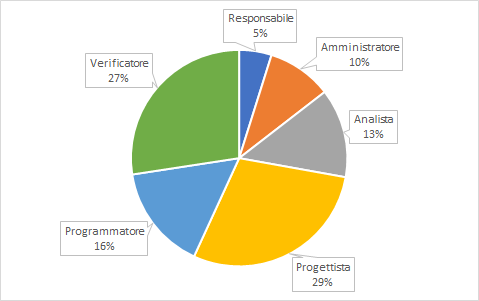
\includegraphics[width=0.7\textwidth]{./res/img/progettazioneArchitetturale_pe.png}
			\caption{Prospetto economico del sedicesimo incremento}
		\end{figure}
	
	\subsubsubsection{Conclusioni}
	
	\subsubsubsection{Preventivo a finire}